\chapter{Monitoring and Logging}\label{monitoring-and-logging}

This chapter shows how to control, monitor, analyze, and visualize
metrics about applications, doing some benchmark to test che scalability
of the apps on this stack.

Monitoring the system resources and logging of applications should be a
first-class task in IT Operations, because it's not possible control
what it's not possible measure. Traditional tools are generally hard to
configure and it needs to create a dedicated transport layer (with
encryption/authentication) of various components between hosts. Luckily,
in this situation it's possible take advantage of the cluster primitives
to make it an easier (and efficient) task.

While \emph{InfluxDB} and \emph{Grafana} are a popular choice
respectively for storage and visualize resource metrics, in logging
world the most popular one is the \emph{ELK} stack, where ELK stands for
\emph{ElasticSearch} (storage), \emph{Logstash} (log processing) and
\emph{Kibana} (visualization). Since a guideline is the lightweight,
instead of using an additional stack for logging, it has been reused
both InfluxDB and Grafana, adding \emph{Heka} for logs processing, so
the stack could be called \emph{IHG}: InfluxDB, Heka and Grafana.

In addition, Kubernetes' kubelet comes with built-in \emph{cAdvisor} for
resource monitoring, while \emph{Heapster} is the main plug-in for
resource cluster manager. At the end, Logspout (built-in in recent
versions of Heka) will be used for gathering logs from all running
containers.

\begin{figure}[htbp]
\centering
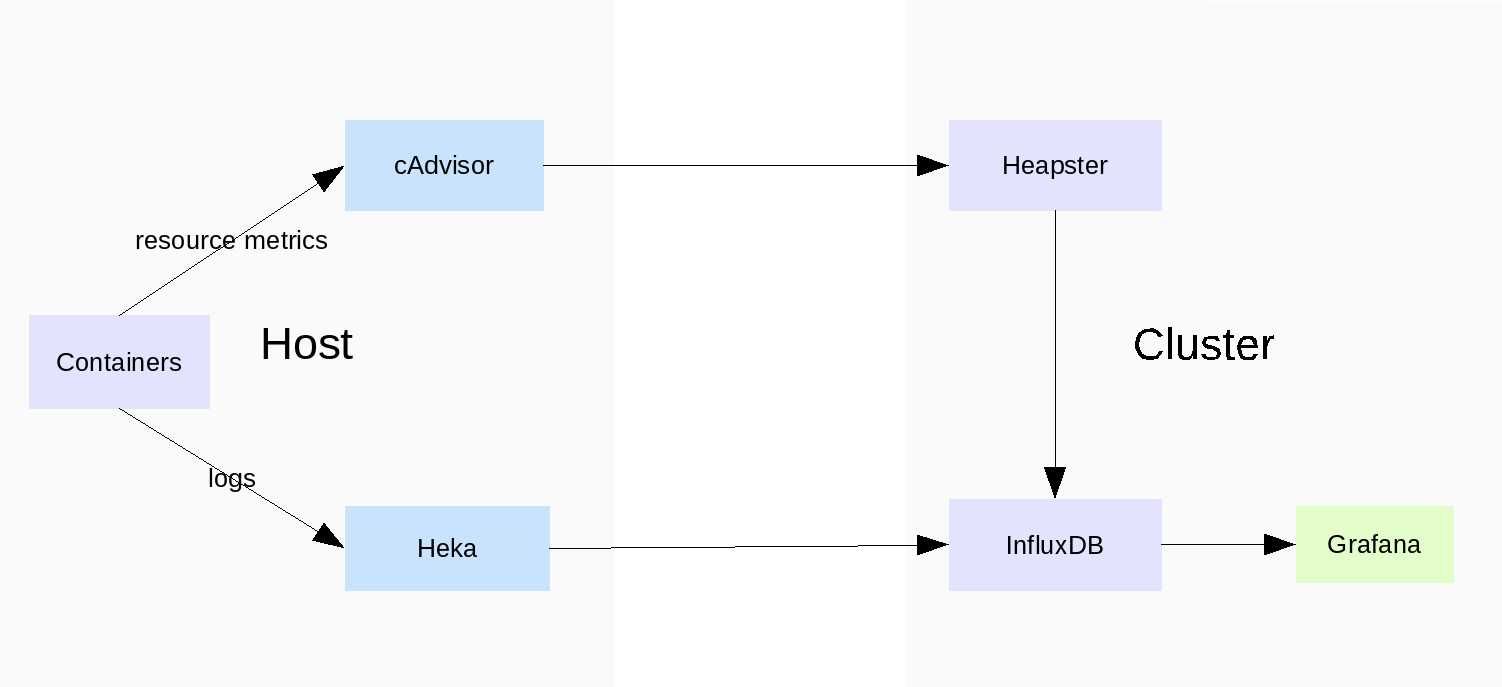
\includegraphics{media/ch6-overview.png}
\caption{Overview of monitoring system}
\end{figure}

The monitoring stack is deployed as an unique application, and includes
\texttt{ReplicationController}s, \texttt{Service}s but also
\texttt{Route}s for external reachability:

\section{Time-Series Storage}\label{time-series-storage}

InfluxDB is a distributed time-series database that fits well since it
doesn't need a pre-defined schema for data, it's horizontally scalable
in the NoSQL way, support native data replication and include a familiar
SQL-like language, \emph{InfluxQL}.

InfluxQL is the query language. Here some examples:

\begin{verbatim}
select * from mem_usage

select * from log_lines where line =~ /error/i

select mean(cpu_load) group by time(30m) where time > now() - 1d and host = 'server E'
\end{verbatim}

Resource:

\begin{verbatim}
[{
  "name": "load_avg",
  "columns": [
    "time",
    "app",
    "value"
  ],
  "points": [[
    1400425342091,
    "Frontend B",
    0.8
  ]]
}]
\end{verbatim}

Log:

\begin{verbatim}
[{
  "name": "log_lines",
  "columns": [
    "time",
    "app",
    "line"
  ],
  "points": [[
    1400425947368,
    "Frontend B",
    "some useful log info"
  ]]
}]
\end{verbatim}

In OpenShift, InfluxDB runs as component of monitoring application, and
is composed by a \texttt{replicationController} and a \texttt{service}:

\section{Resource Gathering}\label{resource-gathering}

Kubernetes comes with built-in cAdvisor
(https://github.com/google/cadvisor) in Kubelet, for resource metrics
gathering, such as CPU, RAM, I/O, network, etc.

Heapster (https://github.com/kubernetes/heapster) is the Kubernetes
cluster monitoring system, that gather metrics from nodes and send them
to InfluxDB.

The exported metrics are:

\begin{itemize}
\itemsep1pt\parskip0pt\parsep0pt
\item
  uptime: Number of milliseconds since the container was started
\item
  cpu/usage: Cumulative CPU usage on all cores
\item
  cpu/limit: CPU limit in millicores
\item
  memory/usage: Total memory usage
\item
  memory/working\_set: Total working set usage. Working set is the
  memory being used and not easily dropped by the kernel
\item
  memory/limit: Memory limit
\item
  memory/page\_faults: Number of page faults
\item
  memory/major\_page\_faults: Number of major page faults
\item
  network/rx: Cumulative number of bytes received over the network
\item
  network/rx\_errors: Cumulative number of errors while receiving over
  the network
\item
  network/tx: Cumulative number of bytes sent over the network
\item
  network/tx\_errors: Cumulative number of errors while sending over the
  network
\item
  filesystem/usage: Total number of bytes consumed on a filesystem
\item
  filesystem/limit: The total size of filesystem in bytes
\end{itemize}

While the exported labels are:

\begin{itemize}
\itemsep1pt\parskip0pt\parsep0pt
\item
  hostname: Hostname where the container ran
\item
  host\_id: Identifier specific to a host. Set by cloud provider or user
\item
  container\_name: User-provided name of the container or full container
  name for system containers
\item
  pod\_name: The name of the pod
\item
  pod\_id: The unique ID of the pod
\item
  pod\_namespace: The namespace of the pod
\item
  namespace\_id: The UID of namespace of the pod
\item
  labels: Comma-separated list of user-provided labels
\item
  resource\_id: Identifier(s) specific to a metric
\end{itemize}

Heapster is deployed as \texttt{replicationController}, a
\texttt{service} and a \texttt{route}.

\section{Log Processing}\label{log-processing}

\emph{Heka} is a framework developed by Mozilla for easy data collection
and processing. Heka is modular and supports mainly 6 different type of
plugins: inputs, splitters, decoders, filters, encoders and outputs. The
first 3 are for gather and parse incoming data to \emph{Heka Message}
standard, the filters parse all theese messages and the later 2 is for
encoding and sending data somewhere else, for storaging or further
processing.

Heka permits to logs parsing, filtering, structuring them and send to
InfluxDB. In this example will use Gasista Felice's NGiNX component for
generating logs and \emph{boom} for doing a lot of requests.

\begin{figure}[htbp]
\centering
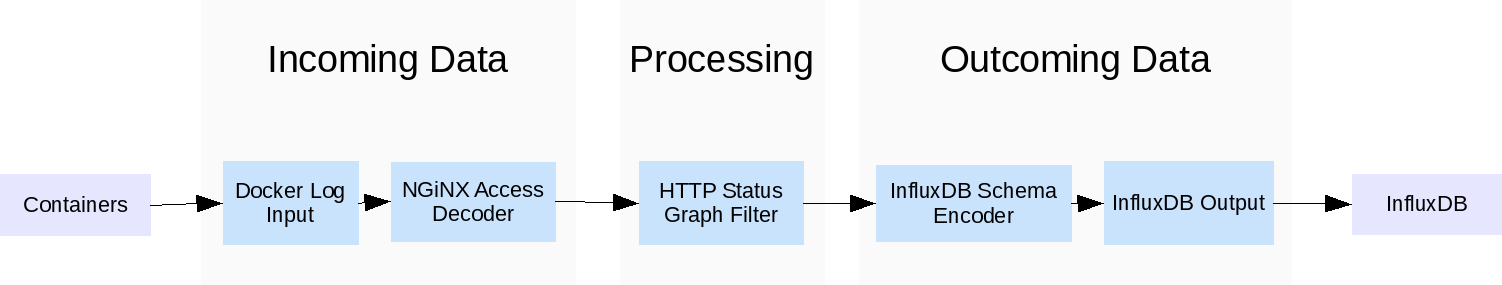
\includegraphics{media/ch6-heka.png}
\caption{The Heka Data Flow}
\end{figure}

The input part is composed by the \emph{Docker Log Input}, build on top
of \emph{Logspout} that acquires stdout/stderr of running containers
from the Docker Engine Unix socket, and \emph{NGiNX access} and
\emph{error decoders}.

Filtering consist of \emph{HTTP Status Graph} that filter NGiNX access
logs and generate an HTTP response code based graph.

The output part is composed by encoding in \emph{InfluxDB schema} and
sending data to \emph{InfluxDB HTTP APIs}.

Heka is deployed on top of OpenShift as a simple
\texttt{ReplicationController}.

\section{Data Visualization}\label{data-visualization}

Grafana is a metrics dashboard and graph editor, born as fork of Kibana
in the beginning of 2014.

\begin{figure}[htbp]
\centering
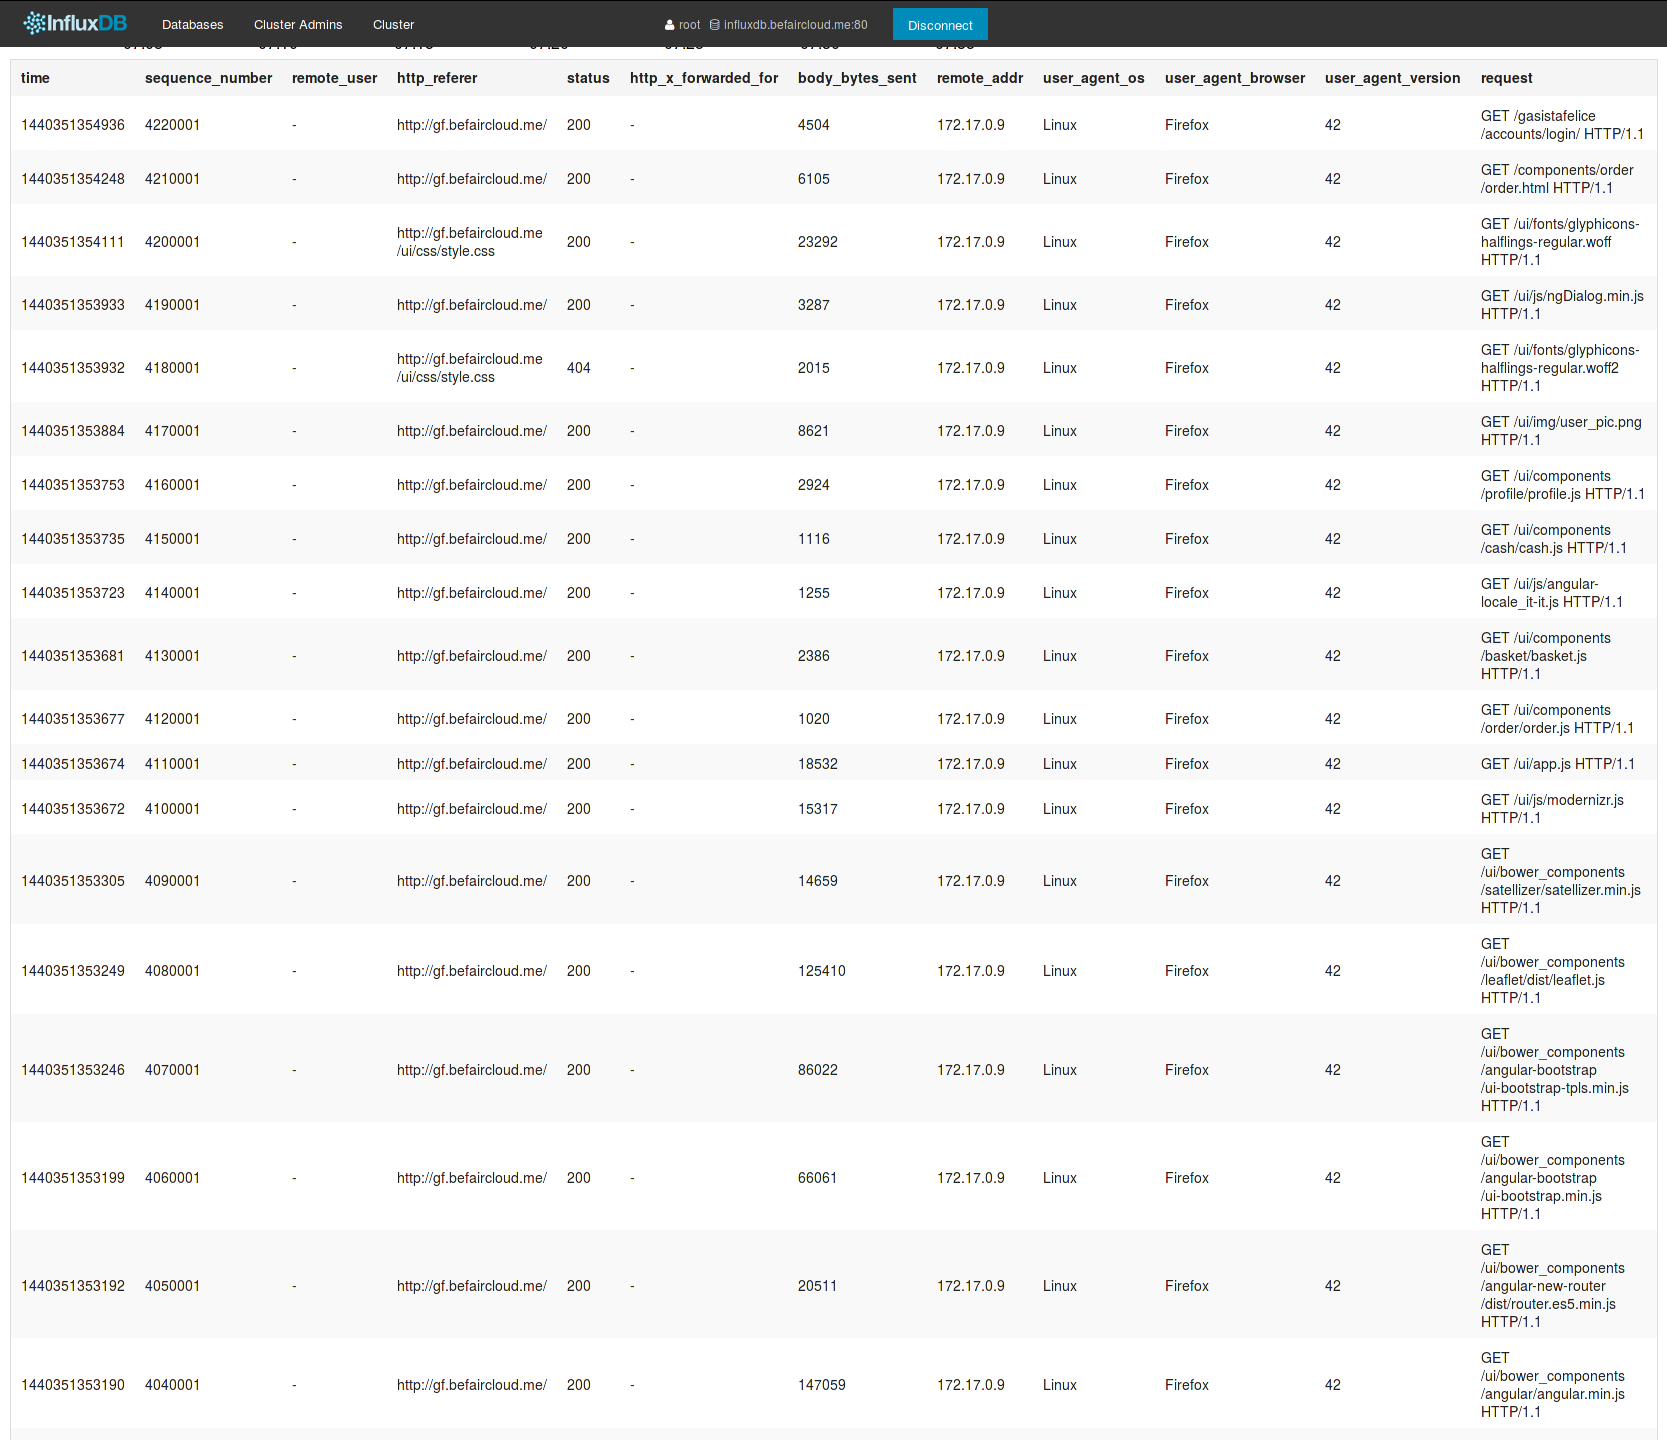
\includegraphics{media/ch6-influxdb.png}
\caption{InfluxDB logs dashboard}
\end{figure}

\begin{figure}[htbp]
\centering
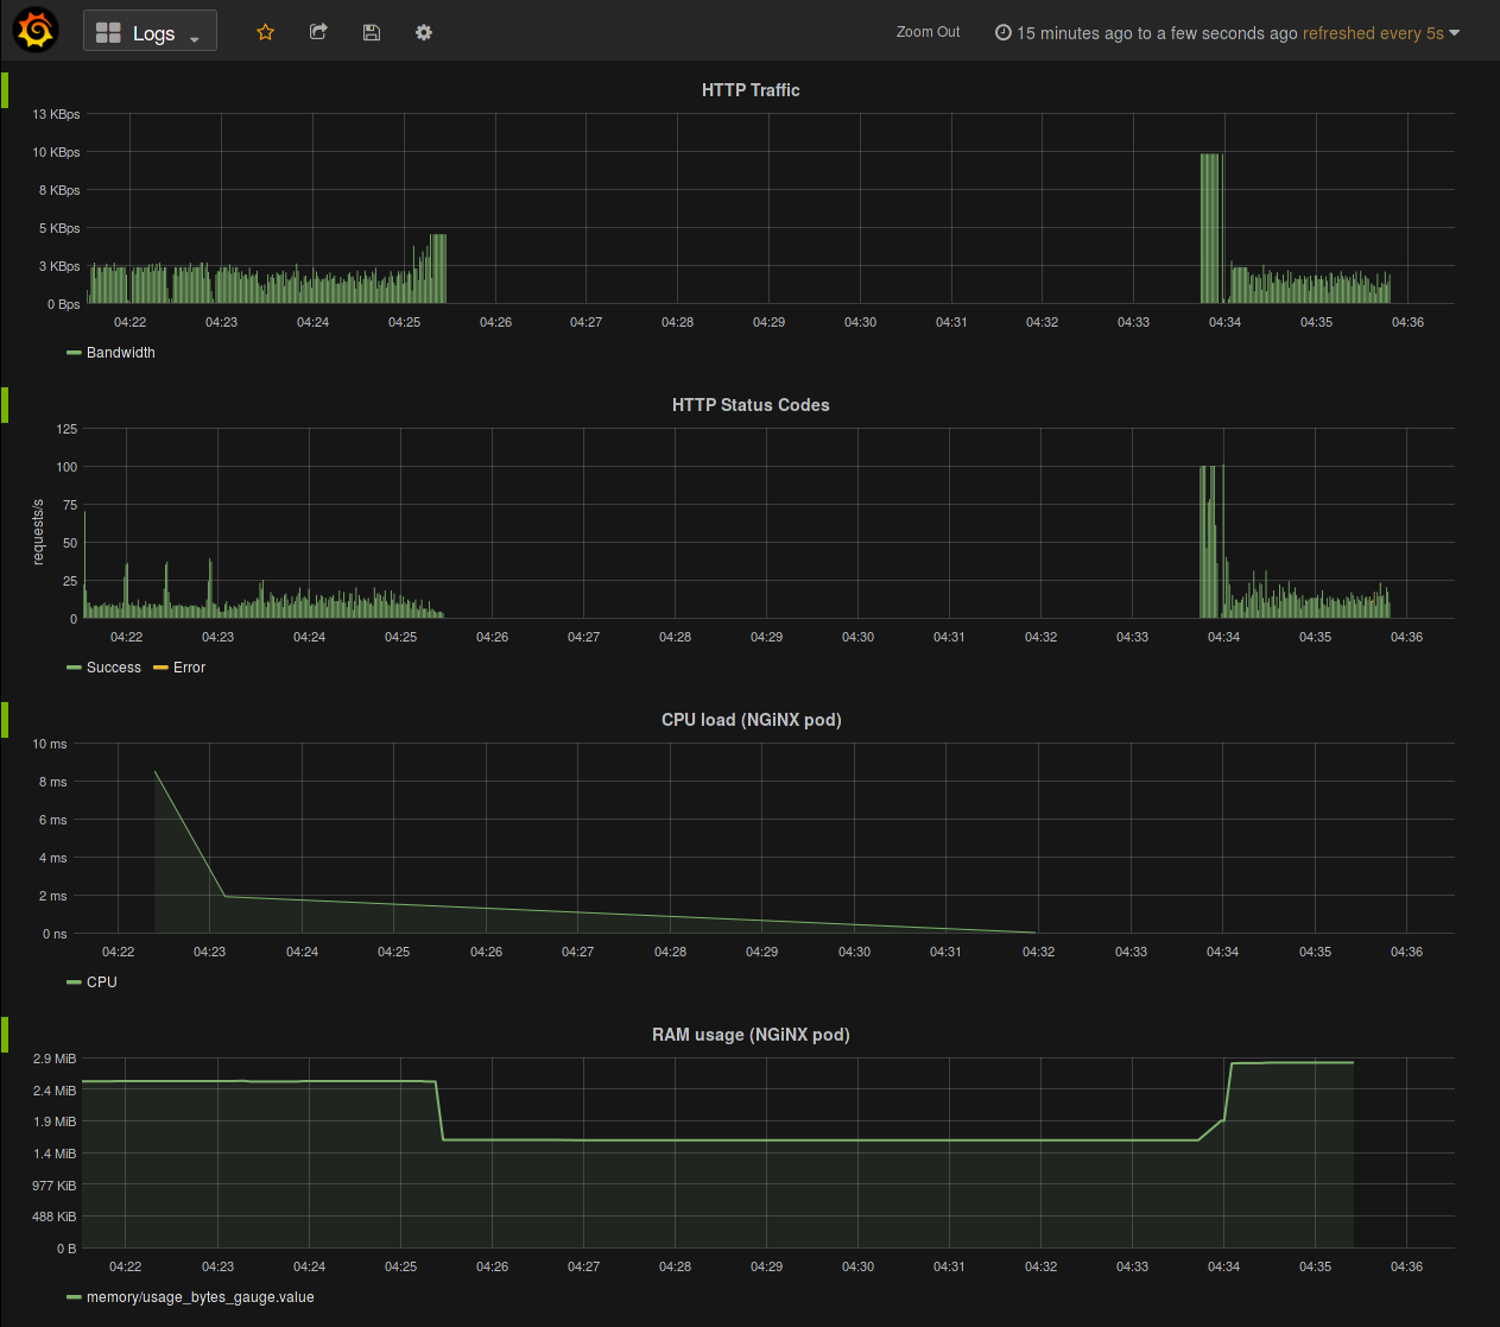
\includegraphics{media/ch6-grafana.png}
\caption{Grafana logs dashboard}
\end{figure}

Grafana is deployed with a \texttt{ReplicationController}, a
\texttt{Service} and a \texttt{Route} in order to be reached from the
external.

\section{Benchmarks}\label{benchmarks}

One of the goal of this project is analyze the component for
scalability. Kubernetes's provide the horizontal scaling of pods, so has
been done some benchmarks varying the number of pods of Gasista Felice
backend.

The test consists in using \emph{boom} for 100 concurrent requests for a
total of 100 requests, that consist in a \emph{GET} at
\texttt{/gasistafelice} path of the application, so a
\texttt{GET\ http://gf.befaircloud.me/gasistafelice} in this case. Even
if this should be a simple request, instead involves several work and
represent a simple but significant test case. The values registered
consist in:

\begin{itemize}
\itemsep1pt\parskip0pt\parsep0pt
\item
  \emph{total time}: interval from the beginning of the first request,
  to the end of the last requests
\item
  \emph{requests per second}: represent the medium of requests served
  per second
\end{itemize}

\begin{longtable}[c]{@{}lll@{}}
\caption{Benchmark results}\tabularnewline
\toprule
Backend pods & total time & reqs/s\tabularnewline
\midrule
\endfirsthead
\toprule
Backend pods & total time & reqs/s\tabularnewline
\midrule
\endhead
1 & 34s & 2.5reqs/s\tabularnewline
2 & 33s & 2.7reqs/s\tabularnewline
3 & 26s & 3.7reqs/s\tabularnewline
4 & 20s & 4.8reqs/s\tabularnewline
8 & 22s & 4.5reqs/s\tabularnewline
\bottomrule
\end{longtable}

The results the decreasing time with adding additional pods, to 4 pods.
Beyond 4 pods there is no advantage, probably because of cluster
resource limit.